% Revision highlights for the adviser (Ms. Eder), 19 Nov 2026.
% Standalone; compile with:  latexmk -pdf adviser-revision-report.tex
\documentclass[11pt,a4paper]{article}
\usepackage[margin=2.2cm]{geometry}
\usepackage[T1]{fontenc}
\usepackage{lmodern}
\usepackage{microtype}
\usepackage{amsmath,amssymb}
\usepackage{booktabs,tabularx,array,longtable}
\usepackage{enumitem}
\usepackage{xcolor}
\usepackage{adjustbox}
\usepackage{float}
\usepackage{tikz}
\usetikzlibrary{positioning,arrows.meta,shapes.geometric,fit,calc,backgrounds}
\usepackage[most]{tcolorbox}
\usepackage[hidelinks]{hyperref}
\newcolumntype{L}{>{\raggedright\arraybackslash}X}
\newcolumntype{P}[1]{>{\raggedright\arraybackslash}p{#1}}
\setlist{itemsep=2pt,topsep=3pt}
\setlength{\parskip}{4pt}
\setlength{\parindent}{0pt}
\setlength{\tabcolsep}{4pt}
\renewcommand{\arraystretch}{1.15}

% same figure fonts and colors as the manuscript (main.tex)
\newcommand{\figfont}{\fontsize{8.5}{10.5}\selectfont}
\newcommand{\figsmall}{\fontsize{7.5}{9}\selectfont}
\definecolor{frozenFill}{gray}{0.94}
\definecolor{frozenLine}{gray}{0.55}
\definecolor{newLine}{RGB}{0,105,120}
\definecolor{newFill}{RGB}{226,243,245}
\definecolor{offLine}{RGB}{190,105,0}
\definecolor{offFill}{RGB}{253,242,226}
\definecolor{noteCol}{RGB}{150,70,0}

% snapshot of manuscript text, with a note on what changed
\newtcolorbox{snap}[1]{enhanced, breakable, colback=frozenFill!60, colframe=frozenLine,
  boxrule=0.5pt, arc=2pt, left=6pt, right=6pt, top=4pt, bottom=4pt,
  fonttitle=\small\bfseries, coltitle=black, colbacktitle=frozenFill, title={#1}}
\newcommand{\changed}[1]{\par\smallskip{\small\color{noteCol}\textbf{What changed:} #1}\par}
\newcommand{\st}[1]{\textbf{#1}}

\title{\textbf{Revision Highlights after the Concept Defense}\\[3pt]
\large A Risk-Calibrated Adaptive Handover Method for Teacher-Guided Flow-Matching Text-to-Speech Inference}
\author{Prepared by Mark Vincent D.\ Limpahan for Ms.\ Marylene S.\ Eder (adviser)}
\date{19 November 2026}

\begin{document}
\section{Further Preliminary Testing Results}

At the concept defense, the proposed method chose a different \emph{switching time} for each utterance: the teacher would stop as soon as its estimate of the final speech had stopped changing (the ``stabilization'' signal), provided the prompt was not noisy (a prompt signal-to-noise check, the ``SNR gate'' at 20~dB). The team then tested this rule in more detail. Table~\ref{tab:findings} lists what the tests showed; the details are in Appendix~D of the manuscript.

\begin{table}[H]
\centering\small
\caption{What the further experiments showed about the concept-defense method (Appendix~D).}
\label{tab:findings}
\begin{tabularx}{\textwidth}{@{}P{4.3cm} L P{4.0cm}@{}}
\toprule
\textbf{Finding} & \textbf{Evidence} & \textbf{What it means} \\
\midrule
The stabilization signal could not show any safe saving & Across six noise levels, calibration with Learn-Then-Test certified no earlier stopping point: 0\% saving, 21 network runs for every utterance & The core signal of the old method did not work \\
Noise fools the stabilization signal & On noisy prompts, the teacher's estimate settles early because it has locked onto the noise (``premature stabilization'') & The signal says ``stop'' exactly when stopping is unsafe \\
The SNR gate misses moderate noise & Prompts with 18--22~dB noise were read as 19.0--24.8~dB and passed the 20~dB gate, giving 86 of 360 (23.9\%) failures, almost five times the 5\% tolerance; a telephone-filtered prompt was read as 44~dB, ``ultra-clean'' & A simple loudness check cannot be the only protection \\
The old failure rule was noisy & Two equally good reference runs disagreed on 22.5\% of the pass/fail labels & The ``added failure'' rule needed redesigning, as the panel also asked (item 18) \\
The real problem on noisy prompts is copied noise & On noisy prompts, the outputs failed because the teacher copied the prompt's background noise into the estimate it handed over, not because it stopped too early & What the teacher hands over matters more than when \\
\bottomrule
\end{tabularx}
\end{table}

The team then tested a different idea (Appendix~E, experiment EXP-034, 30 development speakers, eight prompt conditions). The teacher stops at one fixed point, and when the prompt seems noisy, the noise-carrying values in the teacher's estimate are replaced with values from a quick first attempt by the student. Table~\ref{tab:exp034} compares it with the released DMOSpeech~2 sampler.

\begin{table}[H]
\centering\small
\caption{Development results of the new idea (EXP-034, Appendix~E; 30 development speakers, eight prompt conditions). Higher UTMOS and SIM are better; lower WER is better.}
\label{tab:exp034}
\begin{tabular}{@{}lccccc@{}}
\toprule
\textbf{System} & \textbf{Runs} & \textbf{Time (clean)} & \textbf{UTMOS} & \textbf{WER} & \textbf{SIM} \\
\midrule
New method (router) & 13 & 2.11~s & 2.950 & 0.047 & 0.883 \\
Released DMOSpeech~2 sampler & 21 & 3.41~s & 2.368 & 0.054 & 0.859 \\
Student alone, from its own draft & 3 & 0.51~s & 3.114 & 0.031 & 0.884 \\
\bottomrule
\end{tabular}
\end{table}

What these results show, and what they do not:
\begin{itemize}
\item The new idea was cheaper (13 vs 21 runs, 38\% faster on clean prompts) and better on average than the released sampler, mainly because it did not copy prompt noise.
\item Its new signal (the ``invariant residual'', Section~\ref{sec:components}) recognized the damaged cases far better than the old stabilization signal (detection score 0.864 vs 0.697, where 1 is perfect).
\item On clean prompts only, the released sampler was slightly better on naturalness (UTMOS 3.964 vs 3.891).
\item The student alone (3 runs) was the best on quality. The only reason to keep the teacher is that it gives more varied intonation: the new method kept 96\% of the teacher's added pitch variety on clean prompts, while always correcting kept only 87\%. Whether this variety is worth 10 extra runs is now a planned test (Section~\ref{sec:ch3}).
\item These are development results on few speakers, with a threshold chosen by hand. They justify the change of method; they are not evidence for the final claims, which will come from the calibrated method on new speakers.
\end{itemize}

% =====================================================================
\section{The New Architecture and Its Components}
\label{sec:components}

\subsection*{What stays and what changes}

The released system has a teacher, which turns noise into speech in many small steps, and a student, a faster copy of the teacher that finishes the job. In DMOSpeech~2 the teacher always runs a fixed number of steps and then hands its current estimate of the final speech to the student. Figure~\ref{fig:method} shows the new architecture.

% Figure (Chapter 3 v2): architecture of the risk-calibrated payload router.
% Grey boxes: released DMOSpeech 2 / F5-TTS networks (frozen). Dashed blue
% boxes: components added by the method. Every inference-time box shows its
% forward-pass cost; the total is 13 passes for every utterance.
\begin{figure}[!htbp]
\centering
\begin{adjustbox}{max width=\linewidth}
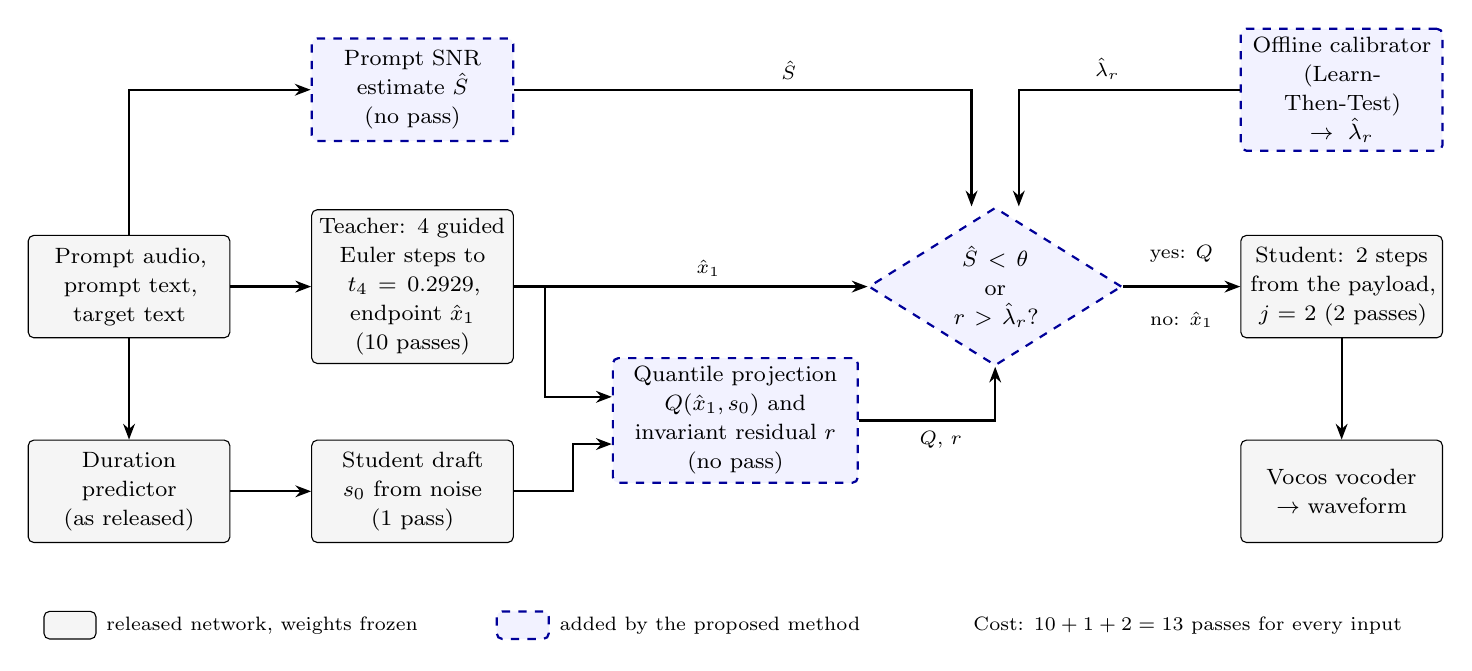
\begin{tikzpicture}[
  font=\figfont,
  base/.style={draw, rounded corners=2pt, fill=gray!8, text width=2.35cm, align=center, minimum height=1.3cm, inner sep=3pt},
  prop/.style={draw=blue!60!black, thick, dashed, rounded corners=2pt, fill=blue!5, text width=2.35cm, align=center, minimum height=1.3cm, inner sep=3pt},
  dec/.style={diamond, draw=blue!60!black, thick, dashed, fill=blue!5, aspect=1.6, inner sep=0pt, align=center, text width=1.55cm},
  arr/.style={-{Stealth[length=2mm]}, thick}
]
% inputs and frozen front end
\node[base] (in)    at (0,0)       {Prompt audio,\\prompt text,\\target text};
\node[base] (dur)   at (0,-2.6)    {Duration\\predictor\\(as released)};
\node[base] (teach) at (3.6,0)     {Teacher: 4 guided\\Euler steps to\\$t_4=0.2929$,\\endpoint $\hat x_1$\\(10 passes)};
\node[base] (draft) at (3.6,-2.6)  {Student draft\\$s_0$ from noise\\(1 pass)};
% added inference-time components
\node[prop] (snr)   at (3.6,2.5)   {Prompt SNR\\estimate $\hat S$\\(no pass)};
\node[prop, text width=2.9cm] (qr) at (7.7,-1.7) {Quantile projection\\$Q(\hat x_1,s_0)$ and\\invariant residual $r$\\(no pass)};
\node[dec]  (route) at (11.0,0)    {$\hat S<\theta$\\or\\$r>\hat\lambda_r$?};
% frozen back end
\node[base] (stud)  at (15.4,0)    {Student: 2 steps\\from the payload,\\$j=2$ (2 passes)};
\node[base] (voc)   at (15.4,-2.6) {Vocos vocoder\\$\rightarrow$ waveform};
% offline calibrator
\node[prop] (cal)   at (15.4,2.5)  {Offline calibrator\\(Learn-Then-Test)\\$\rightarrow\hat\lambda_r$};

\draw[arr] (in) -- (teach);
\draw[arr] (in) -- (dur);
\draw[arr] (dur) -- (draft);
\draw[arr] (in.north) |- (snr.west);
\draw[arr] (teach.east) -- node[above, font=\figsmall, pos=0.55] {$\hat x_1$} (route.west);
\draw[arr] ($(teach.east)+(0.4,0)$) |- ($(qr.west)+(0,0.3)$);
\draw[arr] (draft.east) -- ++(0.75,0) |- ($(qr.west)+(0,-0.3)$);
\draw[arr] (qr.east) -| node[pos=0.3, below, font=\figsmall] {$Q$, $r$} (route.south);
\draw[arr] (snr.east) -| node[pos=0.3, above, font=\figsmall] {$\hat S$} ($(route.north)+(-0.3,0)$);
\draw[arr] (cal.west) -| node[pos=0.3, above, font=\figsmall] {$\hat\lambda_r$} ($(route.north)+(0.3,0)$);
\draw[arr] (route.east) -- (stud.west);
\node[font=\figsmall, align=center] at ($(route.east)!0.5!(stud.west)+(0,0.42)$) {yes: $Q$};
\node[font=\figsmall, align=center] at ($(route.east)!0.5!(stud.west)+(0,-0.42)$) {no: $\hat x_1$};
\draw[arr] (stud) -- (voc);

% legend and cost line
\node[base, minimum height=0.35cm, text width=0.45cm] (l1) at (-0.75,-4.3) {};
\node[right, font=\figsmall] at (l1.east) {released network, weights frozen};
\node[prop, minimum height=0.35cm, text width=0.45cm] (l2) at (5.0,-4.3) {};
\node[right, font=\figsmall] at (l2.east) {added by the proposed method};
\node[right, font=\figsmall] at (10.6,-4.3) {Cost: $10+1+2=13$ passes for every input};
\end{tikzpicture}
\end{adjustbox}
\caption{Architecture of the proposed risk-calibrated payload router. The teacher always stops at the same coarse commit point; the router decides only \emph{what} the teacher hands to the student: its own endpoint estimate $\hat x_1$, or the quantile projection $Q(\hat x_1,s_0)$, which keeps the teacher's timing and uses the student draft's spectral values. The single threshold $\hat\lambda_r$ is set offline by Learn-Then-Test.}
\label{fig:method}
\end{figure}


\begin{table}[H]
\centering\small
\caption{Concept-defense method and new method.}
\label{tab:oldnew}
\begin{tabularx}{\textwidth}{@{}P{3.2cm} L L@{}}
\toprule
& \textbf{Concept defense} & \textbf{Now} \\
\midrule
What adapts per utterance & When the teacher stops (switching time) & What the teacher hands over (payload) \\
Cost & 13 to 21 runs, depending on the utterance & 13 runs for every utterance (released: 21) \\
Decision signals & Prompt SNR; stabilization of the teacher's estimate & Prompt SNR; invariant residual (teacher vs.\ student draft) \\
Failure rule & ``Added failure'' relative to the released output (released assumed failure-free) & One fixed rule for every system, the released system included \\
What is calibrated & Stopping threshold & Correction threshold, with the bound stated against the released system's failure rate \\
Compared with & Fixed switching times; versions of the old rule & Released and published DMOSpeech~2, teacher alone, student alone, and parts of the new method \\
Prosodic variety & Not measured & Measured; it is the reason the teacher is kept \\
\bottomrule
\end{tabularx}
\end{table}

\subsection*{The added components}

\begin{table}[H]
\centering\small
\caption{Components added by the new method and why each was added. Sources are in Table~2.3 of the manuscript.}
\label{tab:newcomp}
\begin{tabularx}{\textwidth}{@{}P{3.3cm} L L@{}}
\toprule
\textbf{Component} & \textbf{What it does} & \textbf{Why it was added} \\
\midrule
Shorter teacher path & Reaches the released handover point in 4 coarse steps instead of 8 & Saves 8 of 21 runs for every utterance; a fixed point avoids the failed stabilization signal \\
Student draft & One quick run of the student from noise & Gives clean reference values; the student does not copy prompt noise the same way \\
Corrected payload (quantile projection) & Keeps the teacher's timing (when sounds rise and fall) but takes the loudness values of each frequency band from the draft & Steady noise changes the values but not their order in time, so this removes copied noise while keeping the teacher's timing \\
Invariant residual & Measures how far the teacher's values have moved from the draft's & Detects copied noise directly in the output, including cases the SNR gate misses \\
Prompt SNR check & Flags clearly noisy prompts, fixed at 20~dB & Cheap first check; no longer the only protection \\
Routing rule & Uses the corrected payload if the prompt is noisy or the residual is above the threshold; otherwise trusts the teacher & Corrects only when needed, which keeps the teacher's variety on clean prompts \\
Calibrator (Learn-Then-Test) & Sets the residual threshold once, on separate speakers & Guarantees, with 90\% confidence, that the method fails on at most 5\% more utterances than DMOSpeech~2; if no threshold passes, DMOSpeech~2 is used unchanged \\
\bottomrule
\end{tabularx}
\end{table}

\subsection*{Concerns we checked, and how the paper handles them}

\begin{enumerate}
\item \st{Does this contradict the concept defense?} Partly it shifts it. The problem stays the same: one fixed handover is applied to every input. What adapts has moved from \emph{when} the teacher stops to \emph{what} it hands over, because our own experiments showed that adapting the timing could not be done safely, while the input-dependent failures came from copied noise. The cost saving now comes from the shorter fixed teacher path, not from adapting. We plan to state this openly in Chapter~1 and in the revision matrix rather than leave the panel to find it.
\item \st{Where is the adaptivity, if every utterance costs 13 runs?} The paper now defines it: the handover is adaptive in its content, not in its amount of computation (Section~1.5 and Section~3.1). A fixed cost also means predictable speed, which matters for real-time and assistive use. Choosing the amount of computation per utterance is stated as outside the scope.
\item \st{Is the teacher worth 10 runs?} In development, the student alone was better on quality. The teacher is kept only for prosodic variety, so the paper fixes in advance one main test: the new method's pitch variety against the student alone, with a small listening check by the team as support. If the variety gain is not shown, the paper will report that the student alone is the cost-effective choice.
\item \st{Why stop the teacher at that point?} The point matches the released handover time. Two other stopping points (10 and 16 runs), the only others where the student can continue exactly where the teacher stops, are added as ablations, so the chosen point can be judged on a cost--quality--variety curve.
\end{enumerate}

% =====================================================================
\section{Novelty of the Proposed Method}
\label{sec:novelty}

The panel asked us to establish where the method comes from (item 9) and how it differs from flow-matching work in image generation (item 22). The answer below separates what we take from earlier work from what is new.

\subsection*{What is not new}
\begin{itemize}
\item \st{Teacher-guided sampling} (teacher first, student finishes) is DMOSpeech~2's.
\item \st{The correction itself}, mapping values onto another set of values while keeping their order, is histogram matching from image processing (Hall, 1974), used since 2000 to remove noise from the inputs of speech recognizers (Dharanipragada \& Padmanabhan, 2000; de la Torre et al., 2005; Hilger \& Ney, 2006).
\item \st{Using disagreement between a large and a small model as a signal} also appears in recent image and video methods (TRACK, HybridStitch, 2026).
\item \st{Learn-Then-Test} is an existing calibration procedure (Angelopoulos et al.), already used for early exit in language models and for speech recognition.
\end{itemize}

\subsection*{What is new}
\begin{enumerate}
\item \st{What is adapted.} Every method we reviewed adapts \emph{how much} computation an input gets: how many steps, which layer to exit at, or when to switch between models. This method keeps the computation fixed and adapts \emph{what} one generative model hands to another. We found no earlier method that does this.
\item \st{A training-free fix for copied prompt noise inside generation.} Recent noise-robust zero-shot TTS methods (Wang et al., 2024; Fujita et al., 2024; Lu et al., 2025) retrain the model or add a trained denoiser. Histogram equalization normalized the input of a recognizer. Here the correction is applied, without any training, to the content passed from teacher to student, and only to the utterances that need it.
\item \st{A disagreement signal that ignores timing.} The invariant residual compares the teacher with the student's draft for each utterance. We prove that it is zero exactly when the two differ only in timing, so it reacts to changed values such as copied noise, not to different but valid timing. TRACK averages disagreement offline into one fixed schedule, and HybridStitch uses hand-set thresholds.
\item \st{A failure bound against the released system.} The calibrated threshold comes with a guarantee that the method fails on at most 5\% more utterances than DMOSpeech~2 itself, with 90\% confidence, and it falls back to DMOSpeech~2 when no threshold passes. Calibrated methods in other fields bound errors of early exit (CALM, thought calibration) or reject samples (FlowGuard); none bounds a teacher-to-student handover in TTS.
\item \st{Proven properties.} The paper proves why the correction removes steady noise and channel effects, what the residual measures, that the cost is fixed at 13 runs, and that the fallback can never be worse than the released system.
\end{enumerate}

\begin{table}[H]
\centering\small
\caption{How the proposed method differs from the closest related work (details in Tables~2.1--2.3 of the manuscript).}
\label{tab:novelty}
\begin{tabularx}{\textwidth}{@{}P{3.6cm} P{2.6cm} P{1.6cm} L P{1.7cm}@{}}
\toprule
\textbf{Approach} & \textbf{What it adapts} & \textbf{Training} & \textbf{Decision signal} & \textbf{Failure bound} \\
\midrule
DMOSpeech~2 & Nothing (fixed) & --- & --- & No \\
Noise-robust zero-shot TTS (2024--2025) & Nothing per input & Retraining or added model & --- & No \\
Histogram equalization in speech recognition & Nothing per input & None & --- & No \\
Large--small switching in image and video (SRDiffusion, TRACK, HybridStitch) & When or where to switch models & None & Change between steps; model disagreement & No \\
Calibrated early exit (CALM, thought calibration, FlowGuard) & When to stop, or whether to reject & None & Confidence; convergence & Yes \\
\textbf{This study} & \textbf{What the teacher hands over} & \textbf{None} & \textbf{Prompt SNR; invariant residual} & \textbf{Yes, against DMOSpeech~2} \\
\bottomrule
\end{tabularx}
\end{table}

The novelty therefore lies in the combination and its use: an existing correction and an existing calibration procedure, joined by a new signal, applied for the first time to the content of a teacher-to-student handover in TTS, with a bound stated against the released system. This claim covers the sources we reviewed; Art is continuing the search, especially for training-free fixes of noisy prompts in TTS.

% =====================================================================
\section{Changes in Chapter 1}

Boxed text below and in Sections~5 and~6 is copied from the manuscript on the group's GitHub \texttt{main} branch as of 19 November 2026 (shortened where marked [\dots]); the orange note under each box says what changed. Only the parts below have changed so far. The background, problem statement, research questions, objectives, significance and definitions still describe the old method and will be rewritten next.

\begin{snap}{Section 1.5, Scope and Limitations (first paragraph)}
This study will focus on developing and evaluating a training-free, risk-calibrated method for choosing, for each utterance, what the teacher hands to the student in teacher-guided flow-matching text-to-speech (TTS), using DMOSpeech~2 and its F5-TTS teacher. In this study, the handover is \emph{adaptive} in its content, not in its amount of computation: every utterance will cost the same number of forward passes, and the method will decide per utterance whether to pass the teacher's own estimate of the output or a corrected version of it. [\dots]
\changed{Before, the study chose the switching time per utterance. The paragraph now defines ``adaptive'' as adaptive in content, so the title still holds.}
\end{snap}

\begin{snap}{Section 1.5, Scope and Limitations (stopping point and measures)}
The teacher will stop at one fixed point for every utterance, the handover time of the released DMOSpeech~2 code, reached in four coarse steps instead of eight, so the method will cost 13 forward passes against the released sampler's 21. Two other stopping points will be tested as ablations, but the stopping point will not be chosen per utterance; making the amount of computation itself depend on the input is outside the scope of this study. [\dots] Speech quality will be measured with automatic measures: word error rate (WER), speaker similarity (SIM), predicted naturalness (UTMOS), and a pitch-based measure of prosodic variety [\dots].
\changed{Before, the switching time was the only setting varied, the student's restart was kept at the released default, and prosodic variety was explicitly not measured. All three are reversed.}
\end{snap}

\begin{snap}{Section 1.6, Conceptual Framework (Figure 1.1)}
Figure~1.1 shows the conceptual framework as input, process and output. The inputs are a speaker prompt, clean or noisy, with the text to be spoken, and a separate group of speakers used only for calibration. The process is the released teacher--student system of DMOSpeech~2, kept unchanged except at the handover. There, the proposed method decides for each utterance whether the teacher passes its own estimate of the speech or a version corrected for prompt noise, guided by two signals and a threshold that is calibrated once. The outputs are speech produced at a fixed, lower cost; a stated limit on how often the method fails where the released system does not; and a threshold, with its procedure, that others can reuse.
\changed{Before, the figure was a detailed architecture that repeated Chapter~3. It is now an abstract view in which only the contribution is highlighted, and the text is one paragraph. The variables table was removed.}
\end{snap}

% Figure: conceptual framework drawn as the architecture of the proposed
% method (Chapter 1). Replaced the input-process-output version, 14 Nov 2026.
\begin{figure}[!htbp]
\centering
\begin{adjustbox}{max width=\linewidth}
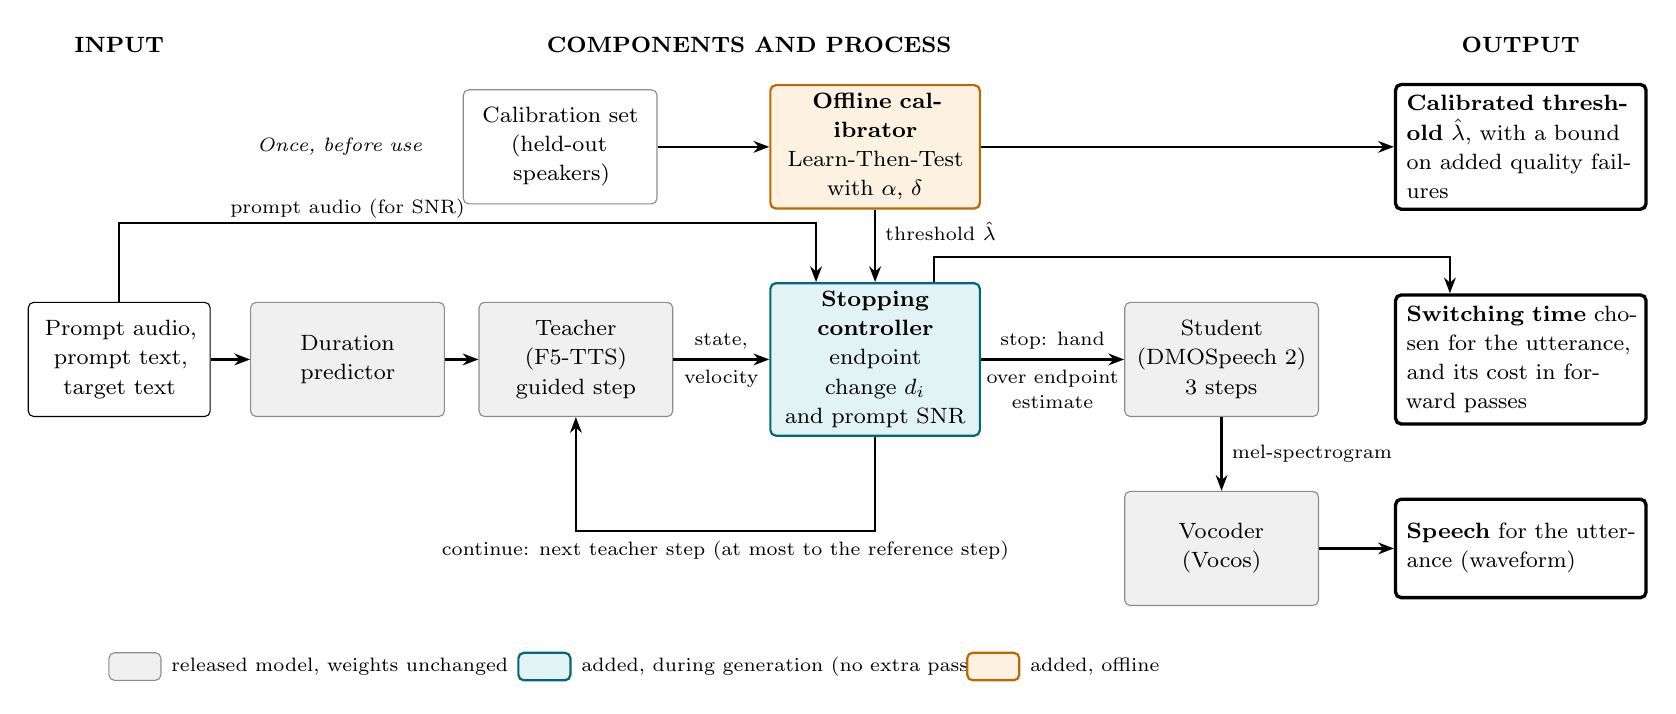
\begin{tikzpicture}[
  font=\figfont,
  frozen/.style={draw=frozenLine, fill=frozenFill, rounded corners=2pt, align=center, text width=2.25cm, minimum height=1.45cm, inner sep=3pt},
  added/.style={draw=newLine, thick, fill=newFill, rounded corners=2pt, align=center, text width=2.45cm, minimum height=1.45cm, inner sep=3pt},
  offl/.style={draw=offLine, thick, fill=offFill, rounded corners=2pt, align=center, text width=2.45cm, minimum height=1.45cm, inner sep=3pt},
  inbox/.style={draw, rounded corners=2pt, fill=white, align=center, text width=2.1cm, minimum height=1.45cm, inner sep=3pt},
  outbox/.style={draw, very thick, rounded corners=2pt, fill=white, align=left, text width=2.9cm, minimum height=1.25cm, inner sep=4pt},
  head/.style={font=\figfont\bfseries, align=center},
  arr/.style={-{Stealth[length=2mm]}, thick},
  lab/.style={font=\figsmall, align=center}
]
% ---------------------------------------------------------------- headers
\node[head] at (0,4.0)    {INPUT};
\node[head] at (8.0,4.0)  {COMPONENTS AND PROCESS};
\node[head] at (17.8,4.0) {OUTPUT};

% ------------------------------------------------- offline row (before use)
\node[frozen, fill=white] (calset) at (5.6,2.7) {Calibration set\\(held-out speakers)};
\node[offl] (cal) at (9.6,2.7) {\textbf{Offline calibrator}\\Learn-Then-Test\\with $\alpha$, $\delta$};
\node[lab, anchor=east, text width=2.6cm] at (4.25,2.7) {\textit{Once, before use}};

% --------------------------------------------- generation row (per utterance)
\node[inbox] (in) at (0,0) {Prompt audio,\\prompt text,\\target text};
\node[frozen] (dur) at (2.9,0) {Duration\\predictor};
\node[frozen] (teach) at (5.8,0) {Teacher\\(F5-TTS)\\guided step};
\node[added] (ctrl) at (9.6,0) {\textbf{Stopping controller}\\endpoint change $d_i$\\and prompt SNR};
\node[frozen] (stud) at (14.0,0) {Student\\(DMOSpeech~2)\\3 steps};
\node[frozen] (voc) at (14.0,-2.4) {Vocoder\\(Vocos)};

% ----------------------------------------------------------------- outputs
\node[outbox] (othr) at (17.8,2.7) {\textbf{Calibrated threshold} $\hat\lambda$, with a bound on added quality failures};
\node[outbox] (osw)  at (17.8,0)   {\textbf{Switching time} chosen for the utterance, and its cost in forward passes};
\node[outbox] (osp)  at (17.8,-2.4) {\textbf{Speech} for the utterance (waveform)};

% ------------------------------------------------------------------ arrows
\draw[arr] (in) -- (dur);
\draw[arr] (dur) -- (teach);
\draw[arr] (teach) -- node[lab, above] {state,} node[lab, below] {velocity} (ctrl);
\draw[arr] (ctrl) -- node[lab, above] {stop: hand} node[lab, below, align=center] {over endpoint\\estimate} (stud);
\draw[arr] (stud) -- node[lab, right] {mel-spectrogram} (voc);
\draw[arr] (voc) -- (osp);
% teacher loop
\draw[arr] (ctrl.south) -- ++(0,-1.2) coordinate (lp) -| (teach.south);
\node[lab, below] at ($(lp)!0.5!(lp-|teach.south)$) {continue: next teacher step (at most to the reference step)};
% prompt audio to the controller (SNR)
\draw[arr] (in.north) |- ($(ctrl.north)+(-0.75,0.75)$) -- ($(ctrl.north)+(-0.75,0)$);
\coordinate (pl) at ($(ctrl.north)+(-0.75,0.75)$);
\node[lab, anchor=south, inner sep=1.5pt] at (pl -| dur) {prompt audio (for SNR)};
% calibration
\draw[arr] (calset) -- (cal);
\draw[arr] (cal) -- node[lab, right, pos=0.3] {threshold $\hat\lambda$} (ctrl);
\draw[arr] (cal) -- (othr);
% switching time and cost
\draw[arr] ($(ctrl.north)+(0.75,0)$) -- ++(0,0.32) -| ($(osw.north)+(-0.9,0)$);

% ------------------------------------------------------------------ legend
\node[frozen, minimum height=0.35cm, text width=0.45cm] (l1) at (0.2,-3.9) {};
\node[right, lab] at (l1.east) {released model, weights unchanged};
\node[added, minimum height=0.35cm, text width=0.45cm] (l2) at (5.4,-3.9) {};
\node[right, lab] at (l2.east) {added, during generation (no extra pass)};
\node[offl, minimum height=0.35cm, text width=0.45cm] (l3) at (11.1,-3.9) {};
\node[right, lab] at (l3.east) {added, offline};
\end{tikzpicture}
\end{adjustbox}
\caption{Conceptual framework of the study, drawn as the architecture of the proposed method. Gray components are the released DMOSpeech~2 sampler with unchanged weights; the stopping controller (teal) decides for each utterance where the teacher stops, and the offline calibrator (orange) sets its threshold before use.}
\label{fig:conceptual}
\end{figure}


\begin{snap}{Theoretical framework (removed for now)}
\textit{Section removed from the manuscript until the Chapter~1 rewrite.}
\changed{It described the old method (stabilization signal, per-utterance stopping) and its figure only restated the method. Dr.~Landicho asked for claims and a framework grounded in TTS principles using existing theory. The proposed replacement: three existing theories, each stated as a TTS principle and tied to one claim: (1) flow matching and teacher-guided distillation; (2) order-preserving normalization and optimal transport, the basis of the corrected payload; (3) distribution-free risk control (Learn-Then-Test). To be confirmed with you before writing.}
\end{snap}

\begin{snap}{Planned reframing of the problem statement (draft, not yet in the manuscript)}
DMOSpeech~2 hands the teacher's work to the student in the same way for every input: the teacher always runs the same number of steps and always passes its estimate unchanged. This fixed handover has two costs. It spends the same teacher computation on every utterance, and on noisy prompts it passes on the noise that the teacher has copied from the prompt. Adapting \emph{when} the teacher stops was the first approach tried; the preliminary experiments showed that no safe saving could be certified that way. This study therefore keeps one shorter teacher path for every input and adapts \emph{what} the teacher hands over, with a calibrated limit on the failures this may add.
\changed{Proposed wording that keeps the concept-defense problem (a fixed handover for every input) and explains why the adaptive part moved.}
\end{snap}

% =====================================================================
\section{Changes in Chapter 2}

\subsection*{Outline, before and after}

\begin{table}[H]
\centering\small
\caption{Chapter 2 outline at the concept defense and now.}
\begin{tabularx}{\textwidth}{@{}P{6.6cm} L@{}}
\toprule
\textbf{Concept defense} & \textbf{Now} \\
\midrule
2.1 Flow-Matching Speech Synthesis and Its Computational Cost & 2.1 Same; the teacher's estimate is now ``the payload''; old curvature passage removed \\
2.2 Methods for Reducing Sampling Cost & 2.2 Same; now states that prosodic variety will be measured \\
2.3 Teacher-Guided Sampling and Re-Noising at the Handover & 2.3 Same title; switching time is fixed background; why the student restarts where the teacher stops \\
--- & \textbf{2.4 Noisy Prompts and Robustness to Recording Conditions (new)} \\
2.4 Input-Adaptive Computation (Table 2.1) & 2.5 Same; Table 2.1 grouped into five categories, with four new methods \\
2.5 Statistical Risk Control and Calibration & 2.6 Same; failures counted against the released system \\
2.6 Evaluation of Zero-Shot TTS & 2.7 Same; UTMOS now in the failure rule; pitch variety and its limits added \\
2.7 Assistive Applications as Motivation & 2.8 Unchanged \\
2.8 Synthesis and Research Gap (Table 2.2) & 2.9 Table 2.2 regrouped by the part of the method each study supports; \textbf{new Table 2.3} on where each component comes from \\
\bottomrule
\end{tabularx}
\end{table}

\subsection*{Blocks changed in response to panel comments}

\begin{snap}{Section 2.4 (new): Noisy Prompts and Robustness to Recording Conditions}
[\dots] All three methods retrain the model or add a trained component. This study instead keeps every network as released and changes only what the teacher hands to the student. [\dots] Speech recognition adopted [histogram equalization] to remove the mismatch between clean training data and noisy test data [\dots]. These methods normalized the inputs of a recognizer; none of them used such a mapping to correct the content that one generative model hands to another, or to decide per input whether a correction is needed.
\changed{New section. It reviews recent noise-robust zero-shot TTS (2024--2025) and the older histogram-equalization work that the corrected payload builds on, and states the gap. Answers items 9 (origin of the method) and 22 (novelty).}
\end{snap}

\begin{snap}{Table 2.1: input-adaptive methods, now in five categories}
Early exit and adaptive depth $\cdot$ Adaptive computation within one model $\cdot$ Handover between a large and a small model (adds SRDiffusion, TRACK, HybridStitch) $\cdot$ Teacher--student collaboration (adds Distillation++) $\cdot$ Calibrated adaptive computation. ``This study'' row: payload handed from teacher to student; prompt SNR and teacher--student residual; calibrated threshold; risk control against the released system.
\changed{Grouped as you suggested. The new large--small methods use the same kind of signal as ours (disagreement between the two models) but give no failure bound. Answers items 12 and 22.}
\end{snap}

\begin{snap}{Table 2.3 (new): Sources of the components added by the proposed method}
Coarse teacher path $\leftarrow$ F5-TTS, step pruning, released code $\cdot$ Student draft $\leftarrow$ DMOSpeech, DMOSpeech~2 $\cdot$ Corrected payload $\leftarrow$ histogram and quantile equalization (Hall 1974; Dharanipragada \& Padmanabhan 2000; de la Torre et al.\ 2005; Hilger \& Ney 2006) $\cdot$ Invariant residual $\leftarrow$ optimal transport; large--small disagreement (TRACK, HybridStitch) $\cdot$ Routing rule $\leftarrow$ early exit (BranchyNet, CALM) $\cdot$ Calibrator $\leftarrow$ Learn-Then-Test $\cdot$ Failure rule $\leftarrow$ CALM, adaptive ASR correction. Each row also says what this study changes.
\changed{New table that answers Dr.~Landicho's ``Where does the method come from?'' (item 9) component by component.}
\end{snap}

\begin{snap}{Section 2.7: UTMOS and the failure rule}
Predicted MOS therefore does not replace listening tests. This study will nevertheless include UTMOS in its failure rule, with a low floor taken from the released system's own scores rather than a small margin, because the payload choice mainly affects naturalness [\dots]. Because this study judges every system, DMOSpeech~2 included, by the same failure rule, the quality and the failure rate of DMOSpeech~2 itself will be measured rather than assumed.
\changed{Before, UTMOS was reported but not used, and failures were counted relative to the released output. Answers items 18 and 21.}
\end{snap}

Other changes: passages tied only to the old stopping rule were removed (learned-path curvature, early-step guidance quotes, FlashSpeech/ZipVoice, step-budget quotes); 18 references were added, each checked against its publisher or arXiv record.

% =====================================================================
\section{Changes in Chapter 3}
\label{sec:ch3}

Chapter~3 was rewritten around the new method. It follows the three objectives (characterize the baseline and the two payloads; develop and calibrate the method; evaluate it), uses future tense, and contains no results. Technical terms are explained when first used, as you asked.

\begin{snap}{Section 3.1, Research Design (second paragraph)}
The method changes only what the teacher passes to the student, not when it passes it. [\dots] The proposed method will stop the teacher earlier, at the same point for every input, and will decide for each sentence whether to pass the teacher's estimate itself or a corrected version of it. The corrected version keeps the teacher's timing [\dots] but takes its loudness values from a quick first attempt by the student, called the student draft. [\dots] The method is therefore adaptive in what the teacher hands over, not in how much computation a sentence receives [\dots].
\changed{Before: ``The experiment will measure how the teacher's switching time affects speech quality and computing cost'' and define a policy that chooses it per utterance.}
\end{snap}

\begin{snap}{Section 3.4.4, Definition 3.1: quality failure}
An output fails if its WER is above 12.5\%, or its SIM is below $s_{\min}$, or its UTMOS is below $u_{\min}$. [\dots] In plain words, an output fails on similarity or naturalness when it is worse than all but the worst 5\% of what the released system produces from clean prompts. [\dots] the released system will itself fail on some inputs, and its failure rate will be measured and reported like every other system's.
\changed{Before, a failure was ``added'' relative to the released output, so DMOSpeech~2 had zero failures by definition. Now one fixed rule applies to every system (item 18), with UTMOS included.}
\end{snap}

\begin{snap}{Section 3.6.1, Problem formulation: what is bounded}
The risk is the share of inputs on which the router fails but the released system does not. [\dots] if the router adds a failure on at most 5\% of inputs, its overall failure rate can be at most 5 percentage points above that of the released system.
\changed{The guarantee is now stated against DMOSpeech~2's measured failure rate, so the comparison with the baseline is direct (items 7 and 18).}
\end{snap}

\begin{snap}{Sections 3.6.3 to 3.6.6: corrected payload, residual and routing rule}
In every band the projection puts the draft's values in the teacher's time order: the frame where the teacher is loudest receives the draft's largest value [\dots]. The draft supplies \emph{which} loudness values the band contains [\dots]; the teacher supplies \emph{when} they occur, which carries its timing and intonation. [\dots] The router uses the corrected payload when the prompt is clearly noisy or when the teacher's values have moved too far from the draft's, and trusts the teacher otherwise.
\changed{New. Each part comes with a short proof of the property it relies on (for example, steady noise cannot change the time order, so the corrected payload is unaffected by it) and a plain-language restatement.}
\end{snap}

\begin{snap}{Section 3.7: calibration}
Before calibration, the failure rule, the tolerance $\alpha=0.05$, the confidence parameter $\delta=0.10$ and the list of candidate thresholds will be fixed. [\dots] The thresholds are tested in the order of the list, and the procedure stops at the first one that is not accepted [\dots]. If even the first threshold is not accepted, no threshold is chosen and the released system is used.
\changed{Same Learn-Then-Test procedure as at the concept defense, now applied to the correction threshold, with DMOSpeech~2 as the safe fallback; $\alpha$ and $\delta$ stated as design choices with reasons (item 10), plus a check at $\alpha=0.10$.}
\end{snap}

\begin{snap}{Section 3.8.1: compared systems (Table 3.10) and comparison matrix (Table 3.11)}
Established systems: released DMOSpeech~2 (21 runs), DMOSpeech~2 paper configuration (30), F5-TTS teacher alone (64), DMOSpeech~2 student alone (4). Proposed: the router (13). Ablations: always correct (13), never correct (12), SNR check only (12--13), router stopping earlier (10) or later (16), student from its own draft (3). Every system will be reported on forward passes, saving, time, WER, SIM, UTMOS, pitch variety, failure rate and excess-failure rate, overall, per prompt condition, and on LibriSpeech-PC.
\changed{Before, the method was compared with fixed switching times and with versions of the old rule. It is now compared with established systems (item 25 and the panel's request to reproduce DMOSpeech~2), and the old stopping rule appears only in Appendix~D.}
\end{snap}

\begin{snap}{Section 3.4.3: prompt conditions and data}
Eight prompt conditions: clean; white noise at 15~dB; white, pink and high-pass noise at 25~dB (moderate); room echo; telephone line; cafeteria babble at 15~dB. Seed-TTS speakers split 100 / 200 / 200 (development / calibration / test), and LibriSpeech-PC test-clean as an unseen dataset, used only for testing.
\changed{Before: clean and 15~dB only, one dataset. Moderate noise and an unseen dataset answer item 23.}
\end{snap}

\begin{snap}{Section 3.8.4: the main test of the teacher's value}
The ten teacher passes of the router are justified only by the variety they add, so one comparison is fixed in advance as the main test of the teacher's value: the router's pitch variety [\dots] against that of the student restarted from its own draft [\dots]. A small listening check by the research team on a fixed subset of these outputs will be reported as supporting evidence only.
\changed{New, in response to the development result that the student alone was better on quality.}
\end{snap}

% =====================================================================
\section{Updated Revision Matrix}

Status: \textbf{Done} = addressed in the manuscript; \textbf{Partly} = addressed in Chapters~2--3 but Chapter~1 or a run is still pending; \textbf{Pending} = not yet done.

{\small
\begin{longtable}{@{}P{0.65cm} P{1.95cm} P{3.9cm} P{6.4cm} P{1.3cm}@{}}
\toprule
\textbf{No.} & \textbf{Panelist} & \textbf{Comment} & \textbf{Action taken} & \textbf{Status} \\
\midrule
\endfirsthead
\toprule
\textbf{No.} & \textbf{Panelist} & \textbf{Comment} & \textbf{Action taken} & \textbf{Status} \\
\midrule
\endhead
\bottomrule
\endfoot
1 & Ms.~Pagal & What is the handover? & Defined in Chapters~2--3 as what the teacher passes to the student at a fixed point; Definition of Terms still uses the old wording & Partly \\
2 & Ms.~Pagal & Sample inputs & Eight prompt conditions defined (Section~3.4.3); actual clean, moderate and very noisy samples still to be produced (R21) & Partly \\
3 & Ms.~Pagal & Does the teacher pass features, gradients or weights? & Only its estimate of the final mel-spectrogram, or the corrected version; no weights or gradients (Sections~2.1, 3.4.1) & Done \\
4 & Ms.~Pagal & Published limit or best value; candidates and features & No study gives a best value; the stopping point is fixed at the released handover time and tested against two alternatives (10 and 16 runs) & Done \\
5 & Ms.~Pagal & Lowest or highest handover that keeps quality? & Reframed: the stopping point is fixed; the method keeps the teacher's estimate as often as the failure bound allows (largest certified threshold) & Done \\
6 & Ms.~Pagal & Metrics and statistical method & Wilcoxon, McNemar, Holm, equivalence tests and bootstrap intervals; significance level separated from $\alpha$ and $\delta$ (Table~3.12) & Done \\
7 & Ms.~Pagal & Basis for a failure & One fixed rule for every system (WER above 12.5\%, or SIM or UTMOS below floors taken from DMOSpeech~2); counted as a rate, never removed (Definition~3.1) & Done \\
8 & Ms.~Pagal & How the two signals are compared & SNR check only, always correct, never correct and the full router compared (Table~3.10) & Done \\
9 & Dr.~Landicho & Where does the method come from? & New Section~2.4 and Table~2.3 trace each component to its sources (summary in Section~\ref{sec:novelty}) & Done \\
10 & Dr.~Landicho & Justify LTT for TTS; $\alpha$ and $\delta$ & LTT needs only pass/fail outcomes, independent inputs and fixed candidates (Section~2.6); $\alpha$, $\delta$ given as design choices with reasons (Section~3.7.3) & Done \\
11 & Dr.~Landicho & Lead with the problem; gap from the RRL & Gap stated in Section~2.9; Chapter~1 problem statement to be rewritten with the reframing above & Partly \\
12 & Dr.~Landicho & Categorize the related studies & Tables~2.1 and~2.2 grouped by category, with a Domain column & Done \\
13 & Dr.~Landicho & Show the saving; define the cap and cost & Cost counted in network runs: 13 vs 21 (38\% fewer) and vs 30 for the paper setting (57\%); time also measured (Table~3.3) & Done \\
14 & Dr.~Landicho & Is 0.25 the best threshold? & DMOSpeech~2 does not test it (Section~2.3); the new stopping point equals the released handover time & Done \\
15 & Dr.~Landicho & Claims; theoretical framework in TTS terms; conceptual framework & Conceptual framework redrawn (Figure~1.1); claims and theoretical framework removed for now, to be rewritten & Partly \\
16 & Dr.~Landicho & Calibration is part of the method; one problem & Calibration is part of developing the method in Chapter~3; Chapter~1 objectives still to be rewritten & Partly \\
17 & Dr.~Landicho & Use the pre-experiment to validate the problem & Appendices~D and~E give the evidence; Chapter~1 to summarize it with the reframing & Partly \\
18 & Dr.~Landicho & Do not set the baseline failure to zero & Same failure rule for DMOSpeech~2; its rate measured; reproduction runs pending (R12) & Partly \\
19 & Dr.~Landicho & Keep the lightweight goal consistent & Fixed lower cost on the Tesla T4; low-end devices as future work (Section~1.5) & Done \\
20 & Dr.~Landicho & Threshold future researchers can use & Calibrated threshold reported with its conditions and the procedure to recalibrate (Section~3.7.4) & Done \\
21 & Dr.~Landicho & Define the metrics and comparison in the RRL & Section~2.7, now including pitch variety and its limits & Done \\
22 & Dr.~Landicho & Novelty against image flow-matching work & Table~2.1 and Section~2.5, with four new large--small methods; novelty summarized in Section~\ref{sec:novelty} of this report & Done \\
23 & Dr.~Landicho & Moderate noise; unseen dataset & Three moderate conditions at 25~dB and LibriSpeech-PC in the design; runs pending (R13) & Partly \\
24 & Ms.~Eder & Working prototype & Prototype updated by Rhenel to the new method (13 runs, live calibration certificate); Appendix~C to be updated (R25) & Partly \\
25 & Ms.~Eder & Comparison matrix against the baseline & Tables~3.10 (systems) and~3.11 (measures); values to come from the runs & Done \\
26 & Ms.~Eder & Back the threshold with literature & CALM, thought calibration and FlowGuard cited (Section~3.7.4) & Done \\
27 & Ms.~Eder & Proposal defense in the first or second week of November & Date to be confirmed with you (R28) & Pending \\
\end{longtable}
}

\section{Task Status and Next Steps}

From the group's task sheet (19 November 2026): 19 of 33 tasks are done, 5 are for checking, 3 are assigned, and 6 are blocked. Three done tasks were completed for the old method and need another pass: R04 (problem statement), which will be redone in the Chapter~1 rewrite; R17 (``lowest handover that keeps quality''), which became item~5 above; and R20 (comparing SNR, stabilization and the full rule), which became the new ablations.

\begin{enumerate}
\item \st{Chapter~1 rewrite} (Mark, with Roxanne): problem statement with the reframing, research questions and objectives for the three stages, claims and theoretical framework, definitions. Unblocks R10, R32.
\item \st{Runs on the Tesla T4} (Rhenel): reproduce DMOSpeech~2 (R12) and the moderate-noise and unseen-dataset conditions (R13); the combined experiments EXP-035/036 are prepared and preregistered but not yet run.
\item \st{Appendices}: Appendices~C (prototype), D and~E still call the old rule ``the Chapter~3 method''.
\item \st{Citations}: three details to confirm (Hall 1974 volume, Dharanipragada \& Padmanabhan 2000 pages, Fujita et al.\ 2024 venue).
\item \st{For your decision:} whether to add ``DMOSpeech~2 with the prompt cleaned by a speech-enhancement model'' as one more compared system (suggested by the recent literature), and the proposal defense date.
\end{enumerate}

\end{document}
